\documentclass{article}
\usepackage[utf8]{inputenc}
\usepackage{amsmath}
\usepackage{geometry}
\geometry{
 a4paper,
 total={182mm,257mm},
 left=14mm,
 top=20mm,
 }
 \usepackage{amsthm}
 \usepackage[utf8]{inputenc}
 \usepackage[italian]{babel}
\usepackage[T1]{fontenc}
\usepackage{amssymb}
\usepackage{physics}
\usepackage{commath}
\usepackage{tikz}
\usepackage{pgfplots}
\usepackage{graphicx}
\graphicspath{ {Immagini/} }
\usepackage{float}
\usepackage{hyperref}
\hypersetup{
    colorlinks=true,
    linkcolor=red,
    citecolor=green
    filecolor=magenta,      
    urlcolor=cyan,
}


%Theorem Environments
\newtheorem{thm}{Teorema}[section]
\newtheorem{lem}[thm]{Lemma}
\newtheorem{property}{Proprietà}[section]
\newtheorem{defn}{Definizione}[section]
\newtheorem{prop}[defn]{Proposizione}
\newtheorem{example}{Esempi}[subsection]
\newtheorem{exerc}[example]{Esercizi Svolti}

%Commandi di Formattazione
\newcommand{\noi}{\noindent}
\newcommand{\note}{\noindent {\quad \bf \underline{Osservazione:}} \quad}
\newcommand{\eg}{\noindent {\bf \underline{Esempio:}} \quad}
\newcommand{\bfemph}[1]{\textbf{\textit{#1}}}
\renewcommand{\emph}[1]{\bfemph{#1}}

%Number Sets
\newcommand{\R}{\mathbb{R}}
\newcommand{\C}{\mathbb{C}}
\newcommand{\Z}{\mathbb{Z}}
\newcommand{\Q}{\mathbb{Q}}

%Shortcuts
\newcommand{\then}{\ensuremath{\Rightarrow}}
\newcommand{\twopartdef}[4]
{
	\left\{
		\begin{array}{ll}
			#1 & \mbox{se } #2 \\
			#3 & \mbox{se } #4
		\end{array}
	\right.
}

%Vectors
\renewcommand{\i}{\vu{i}}
\renewcommand{\j}{\vu{j}}
\renewcommand{\k}{\vu{k}}
\renewcommand{\a}{\va{a}}
\renewcommand{\b}{\va{b}}
\renewcommand{\c}{\va{c}}
\renewcommand{\v}{\va{v}}
\renewcommand{\u}{\va{u}}
\newcommand{\s}{\va{s}}
\renewcommand{\t}{\va{t}}
\newcommand{\verst}{\vu{t}}
\newcommand{\versr}{\vu{r}}
\renewcommand{\r}{\va{r}}
\newcommand{\tauvs}{\vu{\tau}}
\newcommand{\tauvt}{\va{\tau}}
\newcommand{\normvs}{\vu{n}}
\newcommand{\N}{\va{N}}
\newcommand{\g}{\va{g}}
\newcommand{\F}{\va{F}}
\newcommand{\f}{\va{f}}
\newcommand{\M}{\va{M}}
\renewcommand{\l}{\va{l}}
\newcommand{\p}{\va{p}}
\renewcommand{\P}{\va{P}}
\renewcommand{\L}{\va{L}}


\renewcommand{\c}{\overline{c}}
\title{Carrucole}
\author{Roberto Gargiulo}
\date{Ultimo Aggiornamento: \today}


\begin{document}

\maketitle

\begin{prop}[Macchina di Atwood]
La Macchina di Atwood è una macchina composta dalla tipica carrucola ai cui lati sono appesi due corpi.

\begin{figure}[H]
    \centering
    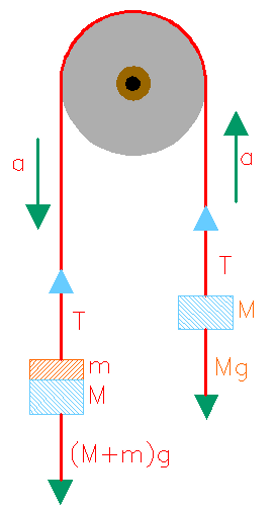
\includegraphics[width=0.25\textwidth]{0650_d1.png}
    \caption{Macchina di Atwood}
    \label{atwoodmachine}
\end{figure}

Dove i corpi hanno massa $m_1,m_2$ rispettivamente e quota $z_1,z_2$ rispettivamente in un riferimento cartesiano centrato nella carrucola (da considerarsi puntiforme) con un asse parallelo al filo e diretto verso il basso. Allora il vincolo della macchina può essere inteso come la lunghezza costante del filo e si può esprimere come segue:
\[f(z)=z_1(t)+z_2(t)-l=0\]
Da cui otteniamo un vincolo per le accelerazioni:
\[\dv[2]{z_1}{t}+\dv[2]{z_2}{t}=0\]
Inoltre per il II principio (posto per comodità $m_2>m_1$ in modo che $a_1<0$):
\[m_1g-|\va{\tau}|=-m_1a_1\quad m_2g-|\va{\tau}|=m_2a_2\]
Otteniamo allora il seguente sistema:
\[\left\{\begin{array}{l}
    a_1(t)+a_2(t)=0  \\
    |\a_1(t)|=a=-g+\frac{|\va{\tau}|}{m_1}\\
    |\a_2(t)|=g-\frac{|\va{\tau}|}{m_2}
\end{array}\right.\]
E quindi l'\textbf{equazione vincolare rispetto alla tensione}:
\begin{equation}
    \boxed{|\va{\tau}|=2g(m_1+m_2)}
\end{equation}
\end{prop}

\begin{prop}
Consideriamo una Macchina composta da due carrucole collegate da un unico filo, una delle quali è mobile ed ha massa non trascurabile, come in figura: 
\begin{figure}[H]
    \centering
    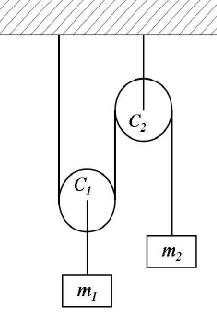
\includegraphics[width=0.25\textwidth]{2i8g76b.png}
    \caption{Carrucola Composta da una mobile e una fissa}
    \label{carrucolamobile}
\end{figure}

Dette $m_1,m_2,m_c$ le masse dei due corpi e della carrucola mobile rispettivamente, allora il vincolo della lunghezza del filo è dato dal sistema:
\[\left\{\begin{array}{l}
    z_2-z_c-l_1=0  \\
    2z_c+z_1-l_2=0 
\end{array}\right.\]
Derivando due volte entrambe le equazioni otteniamo quindi:
\[\left\{\begin{array}{l}
    z_2''(t)-z_c''(t)=0  \\
    2z_c+z_1-l_2=0 
\end{array}\right.\]
\end{prop}

\end{document}
